%
% string matching writeup...
%

\documentclass{llncs}
\pagestyle{empty}
\usepackage{makeidx}  % allows for indexgeneration
%
\usepackage[dvips]{graphicx}    % needed for including graphics e.g. EPS, PS
\usepackage{epsfig}
\usepackage{url}
\usepackage{pseudocode}
\usepackage{comment}
\usepackage{authblk}
\usepackage{color}
\usepackage{newalg}


\begin{document}
\renewcommand{\labelenumi}{(\Alph{enumi})}
\renewcommand{\labelenumii}{(\alph{enumii})}

\frontmatter          % for the preliminaries
%
\pagestyle{headings}  % switches on printing of running heads

\mainmatter              % start of the contributions
%
\title{Bridging the gap: improving local multiple alignment with gapped extension.}
%
\titlerunning{procrastination for local multiple alignment}  % abbreviated title (for running head)
%                                     also used for the TOC unless
%                                     \toctitle is used
\author{Don Quijote}
%
\authorrunning{<Quijote> et al.}   % abbreviated author list (for running head)
\institute{ Castilla La Mancha, Espa\~na }
%
%\institute{ Dept. of Computer Science,
%Univ. of Wisconsin-Madison, USA\\
%\email{darling@cs.wisc.edu},\\
%\and Dept. of Computer Science, Technical Univ. of Catalonia, Barcelona, Spain\\
%\email{treangen@lsi.upc.edu},\\


\maketitle


\begin{abstract}
The identification of homologous DNA via sequence alignment is a basic building block in comparative genomics.  We present a method for accurately and sensitively identifying homologous DNA sequence in multiple genomes. Our method is based around an efficient heuristic for local multiple alignment, featuring a novel method for gapped extensions. In practice, we are able to sensitively identify conserved, potentially repetitive, regions in one or more DNA sequences.  The GPL implementation of our algorithm in C++ is
called \texttt{procrastAligner} and is freely available from
\url{http://gel.ahabs.wisc.edu/procrastination}
\end{abstract}




\section{ Introduction }

Recent advances in sequence data acquisition technology~\cite{ref-454} have provided low-cost sequencing which in turn has
have fueled rapid growth in molecular sequence databases. A central task in comparative genomics is being able to accurately identify all homologous positions in one or more DNA sequences.  Sequence alignment is considered to be the main tool for this task, and specifically, pairwise local alignment has enjoyed a fruitful history in this context.

\subsection{ Pairwise local alignment}
Over two decades ago SW~\cite{ref-sw} introduced an algorithm for optimal pairwise local alignment requiring $O(mn)$ space and time for sequences of lengths $m,n$. While offering an optimal solution, this algorithm was not amenable for large DNA sequences. More recently, a heuristic for local multiple alignment that emphasized speed over sensitivity was presented in  BLAST~\cite{...}, which open the door for rapid homology detection. Several downstream applications have followed, including repeat detection, ...

\subsection{ From pairwise to multiple}
The number of pairwise alignments grows O($n^{2}$) in the copy number of the potentially repetitive region. While this is ok in some cases, IS elements in microbes and Alu elements make local multiple alignment a more attractive option.
Unlike pairwise alignment, local multiple alignment constructs a
single multiple alignment for all occurrences of a motif in one or
more sequences.  Also, local multiple alignments
can identify the basic repeating units in one or more sequences and also 
serve as a basis for downstream analysis tasks such as multiple genome
alignment~\cite{ref-mauve,ref-mga,ref-mgcat,ref-deweyReview}, global
alignment with repeats~\cite{ref-otherSammethPaper,ref-aba}, or
repeat classification and analysis~\cite{ref-piler}. 

\subsection{Previous work}
RepeatScout~\cite{ref-repeatscout}, ABA, ...

%need for a new approach
%To date~\cite{gold}, there are over 500 completed whole genomes in such databases, and in the next few years this number is %expected to reach nearly 3000. To cope with such increases in data volume, corresponding advances in computational methods are %necessary; thus we present an efficient heuristic for local multiple alignment. Our method is based around an efficient %heuristic for local multiple alignment, featuring a novel method for gapped extensions.
\label{sec:overview}
\section{A heuristic for local multiple alignment}
\begin{figure}[t]
\begin{center}
\hfill
\scriptsize
\begin{minipage}[t]{.50\textwidth}
\begin{flushleft}

\begin{enumerate}
\item[\textbf{1.}] \textbf{Detect seeds in DNA sequence(s).}
\begin{enumerate}

\item[1.1] Evaluate palindromic seed pattern at every position in input sequence
\item[1.2] Extract all multi-matches(2 or more) from seeds
\end{enumerate}
%we now have matches
\item[\textbf{2.}] \textbf{Maximal extension of multi-matches}
\begin{enumerate}

\item[2.1] Set extension direction(left or right)
\item[2.2] Perform ungapped extension of all multi-matches to generate chains
\item[2.3] Extend multi-matches in order of decreasing multiplicity 
\item[2.4] Extend each multi-match in current direction(left or right)
\item[2.5] Procrastinate subsets
\item[2.6] If current chain scores above threshold proceed to Step 3.
\end{enumerate}
\item[\textbf{3.}] \textbf{Trigger gapped extension}
\begin{enumerate}
\item[3.1] Perform gapped alignment on region spanning 4*w nucleotides 
\item[3.2] Perform random walk on region to find all high scoring segments
\end{enumerate}
\item[\textbf{4.}] \textbf{Unalign non-homologous sequence}
\begin{enumerate}
\item[4.1] FIXME pairwise homology predictions
\end{enumerate}

\item[\textbf{5.}] \textbf{Determine if boundaries have improved}
\begin{enumerate}
\item[5.1] If original chain boundaries are improved then
return to Step 2, maintaining the current direction.

\item[5.2] else stop extending in the current direction.
\item[5.3] If finished extending in both directions, then
finalize chains, i.e. remove overlaps and align gaps


\end{enumerate}
%we now have local multiple alignments
\item[\textbf{6.}] \textbf{Scoring final local multiple alignments}
\begin{enumerate}
\item[6.1] FIXME
\end{enumerate}
\item[\textbf{7.}] \textbf{Assigning significance to local multiple alignments}
\begin{enumerate}
\item[7.1] FIXME
\end{enumerate}

\end{enumerate}

\end{flushleft}
 \end{minipage}
 \hfill
 \begin{minipage}[t]{.30\textwidth}
 \begin{flushleft}  
\epsfig{file=./figures/flowchart.eps,width=1.8in}

\end{flushleft}  
\end{minipage}
\hfill
\end{center}
\caption{Overview of the method}
\end{figure}
\begin{figure}[t]
\centering \epsfig{file=./figures/extension.eps,width=4.5in}
\caption{.}

\label{fig:string_matching}\vspace{-0.2cm}
\end{figure}

%maybe this could be useful...
\begin{comment}
\begin{algorithm}{Allocate-Object}{}
\begin{IF}{free = \NIL}
\ERROR{out of space}
\ELSE
x \= free \\
free \= next[x] \\
\RETURN x
\end{IF}
\end{algorithm}
\end{comment}


%\colorbox[named]{Gray}{adfa}



\subsection{Notation}
Given a sequence $\mathcal{S}=s_1, s_2,\dots, s_N$ of length $N$
defined over an alphabet $\{A,C,G,T\}$, our goal is to identify all homologous
local multiple alignments on subsequences of $\mathcal{S}$. We denote
an ungapped alignment, or match, among subsequences in $\mathcal{S}$
as an object $M$.  We refer the number of regions in $\mathcal{S}$
matched by a given match $M_i \in \mathbf{M}$ as the
\textit{multiplicity} of $M_i$, denoted as $|M_i|$. We denote
a gapped alignment over an alphabet $\{A,C,G,T,-\}$ as $A$. 

\subsection{Generating candidate multi-matches using a palindromic seed patterns.}

As a starting point for homology detection, we locate all spaced seeds of a given weight $z$ in the input sequence(s). The palindromic spaced seed pattern is analyzed at each position in the input sequence to identify all multi-matches.  Previously we have demonstrated that palindromic spaced seeds offer good efficiency and sensitivity on a variety of input sequences~\cite{ref-procrast}. 

\subsection{Maximal extension of all multi-matches}

Once we have generated a list of multi-matches, we rely on our previously described method for efficient filtration method for maximal extension and chaining~\cite{ref-procrast}. 


\subsection{Gapped Extension of all chains}
We would like to perform gapped
extension to detect all surrounding homologous sequence. Finding boundaries of sequence homology is a difficult and unsolved problem. We here present a novel heuristic for estimating boundaries of sequence homology, and we are very meticulous to avoid classify non-homologous DNA positions as homologous.


\subsubsection{Gapped alignment via MUSCLE}
We employ MUSCLE to perform gapped alignment in the regions surrounding the chains. We try extending 4*w nucleotides to the left/right of each chain. However, we only trigger gapped alignment if chain is above some minimum score threshold. This idea has been used in other local multiple alignment heuristics in order to minimize the number of gapped extensions that do not improve the boundaries of the chain. We score the resulting gapped alignment via sum of pairs. We continue to perform gapped alignment to the left/right) until we reach a score(calculated by sum of pairs) that has been previously determined via simulations to be non-homologous. i.e. a record height in the score signals the start of a stretch of non-homologous sequence.  If we improve our original seed boundaries we then trigger another round of extension, else we stop. 


\subsubsection{Random walk to extend homology border}
FIXME
\begin{itemize}
\item after scoring each column of the gapped extension, we would like
to determine where the homology ends/begins in this region
\item we do this by performing a random walk of the cumulative column score
\item we stop when we reach the record height
\item we determine the record height by simulations
\item all high scoring segments in the gapped extension are reported
\item if boundaries of the original chain are improved, trigger another round of extension.
\end{itemize}

\subsubsection{Processing Novel homologous sequence}
\begin{itemize}
\item novel homologous sequence can be found during gapped extension
\item should briefly describe what we do with this
\end{itemize}
\subsection{Unaligning non-homologous sequence}
FIXME
\begin{itemize}
\item our extension is not quite finished yet. Everything ok so far except that we could
still be including non-homologous sequence in our extended chain(local multiple alignment).
\item Define sets/subsets/boundaries with a pairwise homology test
\item first, we unalign any non-homolgous sequence introduced during the extension process
\item then, we define common boundaries among all sequences in the alignment
\end{itemize}
\subsection{Scoring the local multiple alignments}
Ideally, once our algorithm finishes we will have a complete listing of all homologous local mulitple alignments. This list could be potentially overwhelming, and even at this point, we still need a way of selecting only the highly significant alignments. 

\subsection{Assigning significance to the scores}
FIXME
basically want to extend blast statistics to multiple local alignment. How?
\begin{itemize}
\item Extending Repseek simulations to multiple
\item Tompa et al, estimating the parameters for multiple alignments
\item will involve running procrastAlign with fixed parameters on sequences varying in composition and length
\item also will have to take into account multiplicity
\item FIXME: fill in more details on Monday
\end{itemize}

\section{Results}
We have created a program called \texttt{procrastAligner} for Linux,
Windows, and Mac OS X that implements the described algorithm. Our
open-source implementation is available as C++ source code licensed
under the GPL.

\subsection{Limitations}
%limitations
\begin{itemize}
\item Not really useful for detecting subtle motifs such as transcription factor
binding sites in small, targeted sequence regions
\item Memory bottleneck for large sequences
\item palindromic spaced seeds not ideal for more diverged sequence.
\end{itemize}

\subsection{Comparison with previous version of procrastAligner I}
\begin{table}[t]
  \centering
\begin{tabular}{lccccccccccc}
\hline Accession & Length & Rep & Family & Alu (bp) & Div, \% & Method & Sn \% & Sp \% & T (s) & Sw & $w$ \\
\hline
\hline AF435921 &  22 Kb &  28 & 10 & 261 (69) & 15.0 (6.4) & procrast & 100 & 95.9 & 1 & 9 & 27 \\
\cline{7-12}                                            &&&&&& procrastII & 100 & 94.7 & - & 9 & 27 \\
\hline Z15025 &    38 Kb &  52 & 13 & 245 (85) & 15.7 (5.7) & procrast & 100 & 82.5 & 2 & 9 & 27 \\
\cline{7-12}                                            &&&&&& procrastII & 100 & 77.5 & - & 9 & 27 \\
\hline AC034110 & 167 Kb &  87 & 18 & 261 (72) & 12.2 (5.9) & procrast & 100 & 97.9 & 3 & 15 & 45\\
\cline{7-12}                                            &&&&&& procrastII & 100 & 99.7 &- & 15 & 45 \\



\end{tabular}
\vspace{0.1cm}
  \caption{Performance of \texttt{procrastAlign}, and  \texttt{procrastAlignII} on Alu repeats.
  Rep: total number of Alu elements; Family: number of Alu
  families; Alu: average Alu length in bp (S.D.); Div: average Alu divergence (S.D.);
   Sn: sensitivity; Sp: specificity; T: compute time; Sw: palindromic seed weight; $w$: max gap size.  Alus were
  identified by RepeatMasker~\cite{ref-repbase}.}
  \label{table:alu}
\end{table}

 \subsection{Comparison with RepeatScount}
\begin{itemize}
\item Number and total length of repeat families in our RepeatScout
library versus Repbase Update (Jurka, 1998, 2000) for human, mouse
and rat. Taken from Table 2 from paper.
\end{itemize}

\subsection{Comparison of gapped
extension approaches}
\begin{itemize}

\item RepeatScout extends one nucleotide at a time
\item ABA merges pairwise matches and resolves inconsistencies by
whorl and bulge removal
\item multiz? and HomologMiner? also merge pairwise matches, how do
they resolve inconsistency?
\item procrastAligner generates multiple alignments using libMUSCLE,
which does progressive multiple alignment.  Progressive means that
pairwise alignments do enter in at some stage, but for higher
multiplicity matches, much of the alignment is multiple alignment.
cite a paper which shows multiple alignment is more accurate than
pairwise alignment.  MUSCLE's iterative refinement procedure ensures
a high-scoring alignment irrespective of guide tree.

\end{itemize}

\subsection{Run on new data}
 \begin{itemize}
 \item Ocean metagenomic data(6.4 GB)
 \item Detecting large segmental duplications(dispersed \& tandem)
\end{itemize}

\section{Discussion}

\section{ Acknowledgments }
AED was supported by NLM Training Grant 5T15LM007359-05. TJT was
supported by Spanish Ministry MECD Grant TIN2004-03382 and AGAUR
Training Grant FI-IQUC-2005.

\bibliographystyle{splncs}
\small
\bibliography{procrastination}


\end{document}
